\subsection{Results}
\subsubsection{Temperature gradients}

\begin{figure}[H]
	\centering
	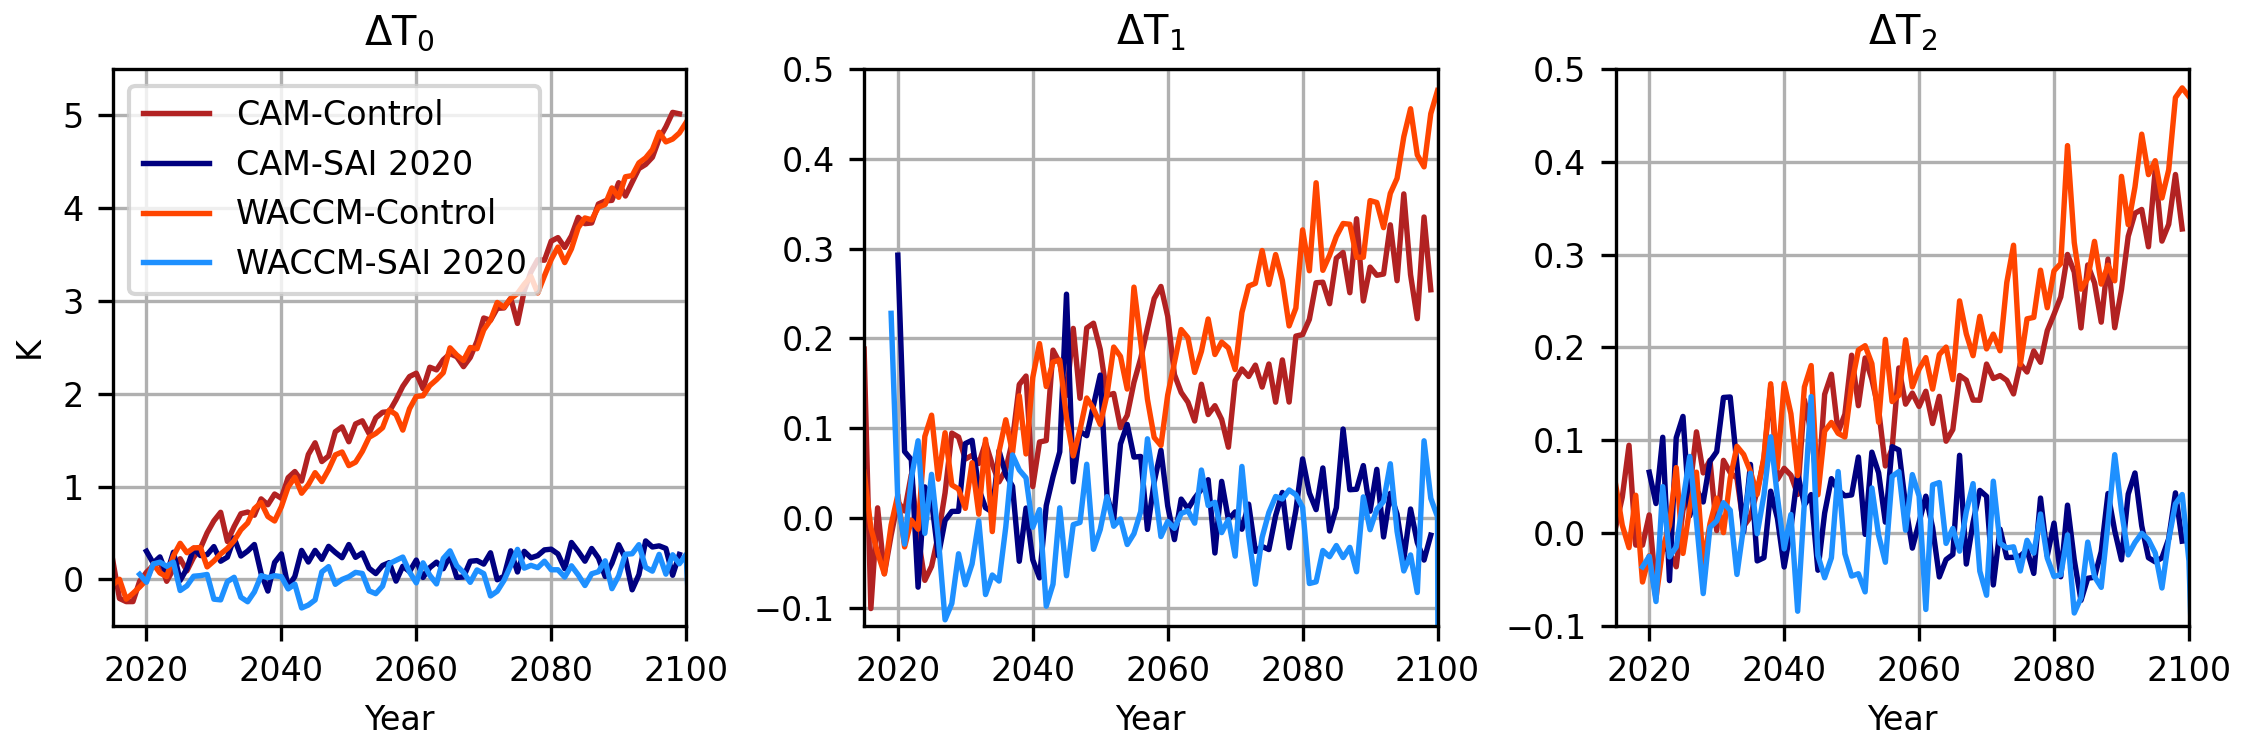
\includegraphics[width=\linewidth]{/Users/Simone/Documents/Uni/Master/Y2/Thesis/Paper_imgs/png/Tgrad_2.png}
	\caption{Temperature gradients $T_0$, $T_1$, $T_2$ as compared to 2016-2025 mean, for Control and SAI 2020 scenarios in CAM and WACCM}
	\label{fig:Tgrad}
\end{figure}

The surface temperature gradients as described by Kravitz et al. are shown in Figure \ref{fig:Tgrad}, we learn:
\begin{itemize}
	\item The global mean surface temperature $T_0$ is very comparable in both scenarios between the models.
	\item Pole-to-pole gradient $T_1$ shows similar behaviour in both the Control and SAI 2020 scenario.
	\item Early-mid century CAM-SAI 2020 possibly more variability compared to WACCM-SAI2020, late century very similar.
	\item Inter-hemispheric temperature $T_2$ also shows very similar behaviour in both scenarios. 
	
	\item Even though our model only corrects for $T_0$, the behaviour of $T_1$ and $T_2$ is still highly comparable to the WACCM experiment that corrects for all three. Our method in CAM emulates the WACCM experiment very well. 
\end{itemize}

\subsubsection{General performance maps}

\begin{figure}[H]
	\centering
	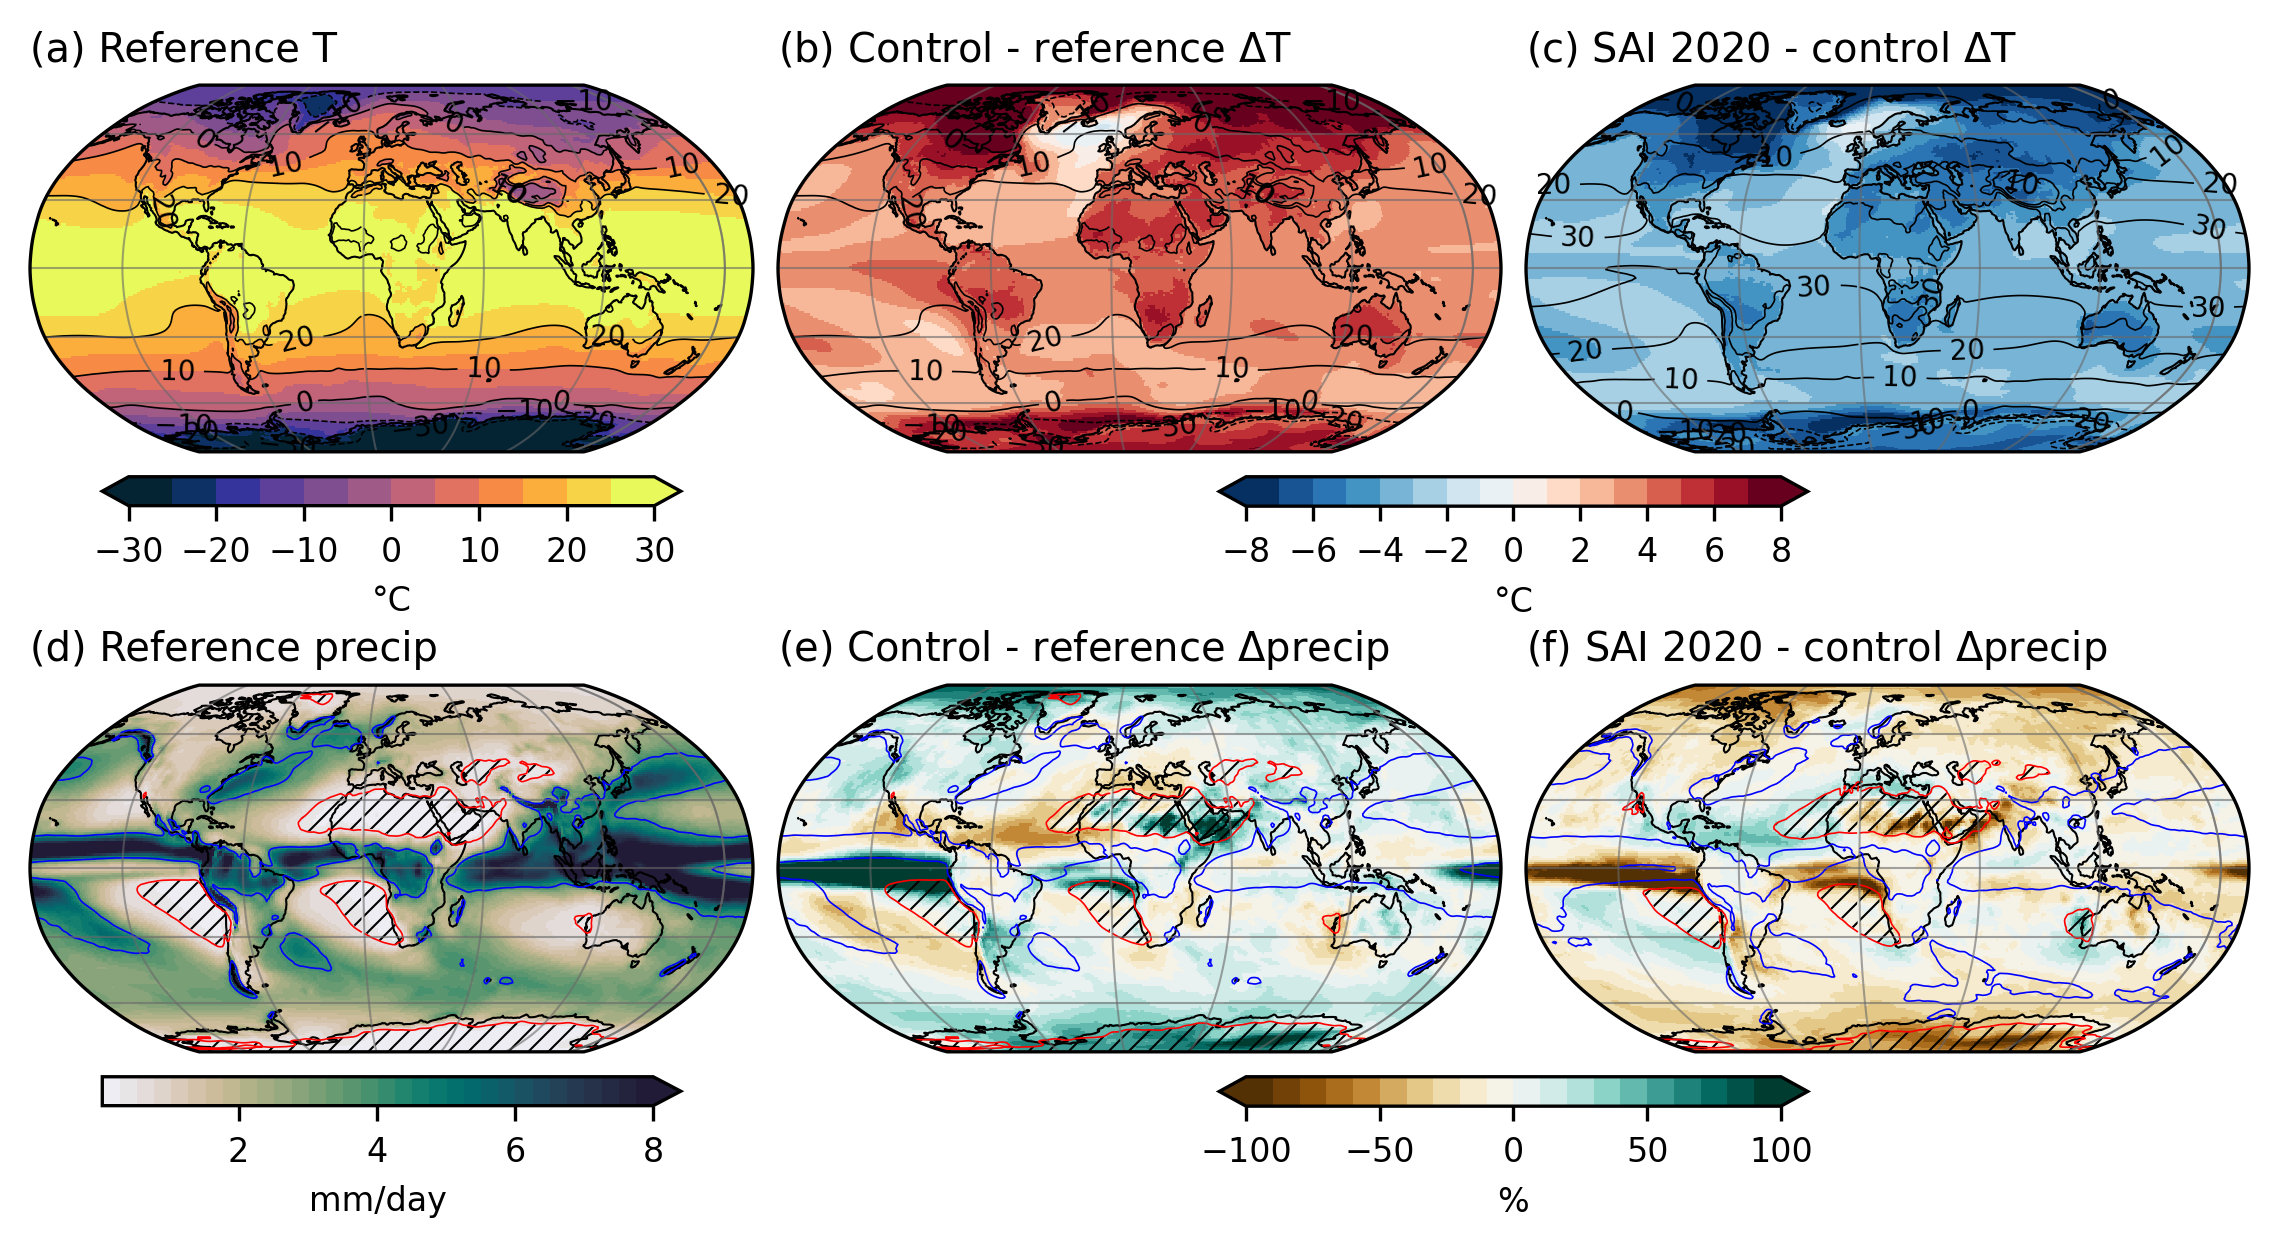
\includegraphics[width=\linewidth]{/Users/Simone/Documents/Uni/Master/Y2/Thesis/Paper_imgs/png/CAM_scens.png}
	\caption{(a): Reference annual mean reference height temperature. (b): Annual mean eference height temperature anomaly for Control compared to Reference, Reference shown in black contours in 10°C intervals. (c): Annual mean reference height temperature anomaly for SAI 2020 compared to Control, Control shown in black contours in 20°C intervals. (d): Reference annual mean precipitation in mm/day, 4 mm/day shown in blue contours, $<0.3$mm/day shown in red contours with hatching. (e) Annual mean precipitation anomaly for Control compared to Reference. Contours as in (d). (f): Annual mean precipitation anomaly for SAI 2020 compared to Control. Contours as in (d) but for Control.}
	\label{fig:CAM_map}
\end{figure}

The surface temperature gradients as described by Kravitz et al. are shown in Figure \ref{fig:CAM_map}, we learn:
\begin{itemize}
	\item (b) shows expected pattern, overall large temperature increase, polar amplification and retreat of Antarctic sea ice, warming hole over North Atlantic. 
	\item (c) shows SAI 2020 prevents most warming, especially polar amplification, warming hole still present and Antarctic sea ice largely preserved. 
	\item (e) shows equatorward shift of ITCZ in pacific, drying over mid-atlantic ITCZ, increase in some dry areas like Sahara and Antarctica.
	\item (f) shows shift of pacific ITCZ somewhat prevented, as well as drying over mid-atlantic ITCZ, overall patterns reversed. 
\end{itemize}

\subsubsection{Reference Height Temperature}

\begin{figure}[H]
	\centering
	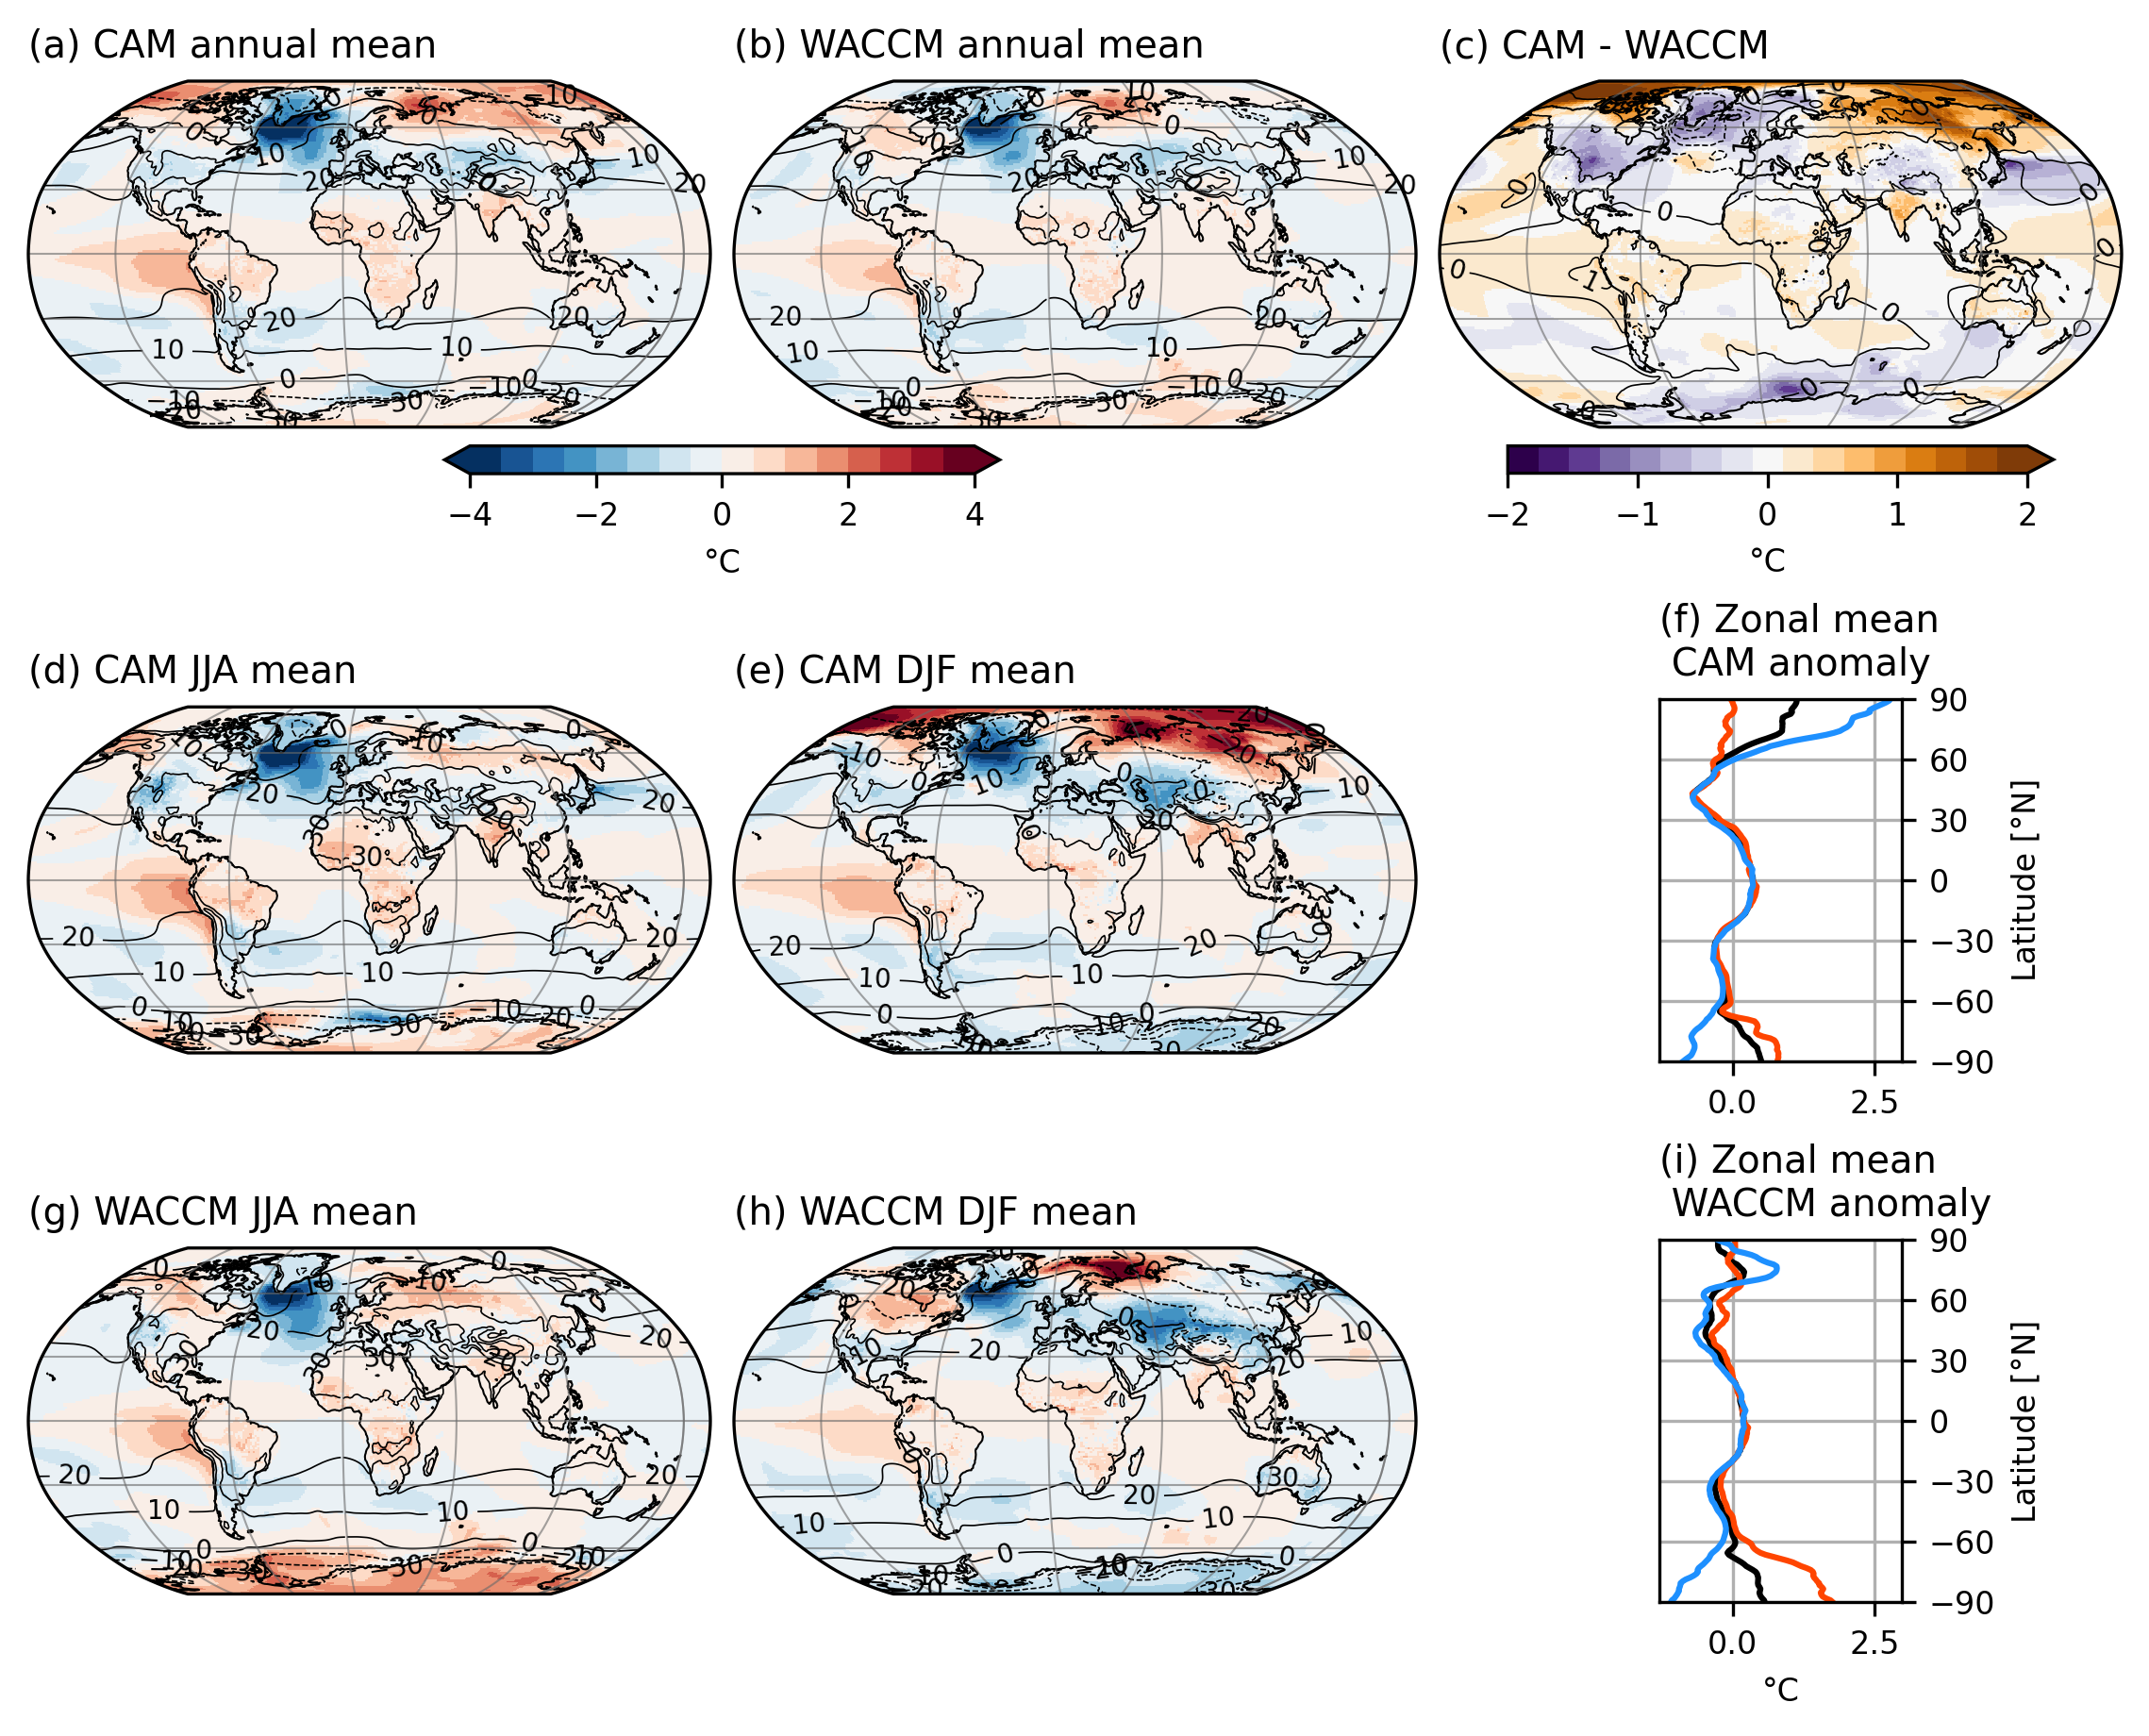
\includegraphics[width=\linewidth]{/Users/Simone/Documents/Uni/Master/Y2/Thesis/Paper_imgs/png/TREFHT_20ref.png}
	\caption{(a,b): Annual mean reference height temperature anomalies of SAI 2020 compared to Reference in (a) CAM and (b) WACCM. Reference mean temperature shown in black contours in 10°C intervals. (c): Difference between CAM and WACCM temperature anomalies. WACCM anomaly shown in black contours in 1°C intervals. (d,e): CAM anomalies as in (a,b) for (d) JJA and (e) DJF. (f): CAM zonal average temperature anomaly as in (a,b), annual mean anomaly in black, JJA anomaly in red, DJF anomaly in blue. (g,h,i): analogous to (d,e,f) for WACCM.}
	\label{fig:TREFHT}
\end{figure} 

The annual mean reference height temperature anaomalies are shown in Figure \ref{fig:TREFHT}, we learn:

\begin{itemize}
	\item Spatial patterns of warming and cooling generally similar, warming over equator (especially eastern Pacific), cooling in subtropics, warming over the poles.
	\item Warming hole over North Atlantic present in both models, due to AMOC collapse in POP2 ocean model used for both CESM2 simulations. Any variations in this model possibly due to differing fresh water fluxes over whole ocean (Claudia zei dat Henk dit was tegengekomen?)
	\item CAM shows clear warming in the Arctic ($>$1°C), slight warming in the Antarctic ($<$1°C)
	\item WACCM only shows significant warming over Barentsz sea ($>$1°C) and similar warming over the Antarctic compared to CAM.
	\item CAM warms more than WACCM in most of the Arctic, excluding Greenland. Tropics also experience slightly more warming in CAM.
	\item CAM cools more than WACCM in Greenland/North Atlantic, North America, Northwest Pacific and Southern Ocean South of Africa. Les clearly so on Tibetan Plateau.
	
	\item In \textbf{JJA} the warming hole is the largest anomaly for both CAM and WACCM, showing slight differences in intensity but overall similar extent.
	\item WACCM shows significantly more warming than CAM over the whole of the Antarctic, also represented in the zonal mean anomaly. WACCM shows slightly more warming over Western Siberia and Norhtern Canada. 
	\item CAM shows more warming than WACCM over the Eastern Pacific, mainly showing warming over an much larger extent. CAM shows slightly more warming over Alaska, Western Africa and South Asia. 
	\item in \textbf{DJF} the warming hole is still present in both CAM and WACCM, again larger extent and more intense in CAM. 
	\item WACCM shows slightly more warming than CAM in the interior of Canada/Hudson Bay and slightly more cooling over Central Asia. 
	\item CAM shows much more warming of the Arctic and Eastern Siberia than WACCM, also represented in the zonal mean anomaly. CAM shows slightly more warming over the Eastern Pacific again, as it does in JJA.
	
	\item Most of the differences observed between WACCM and CAM are attributable to the winter months in the respective hemispheres. 
	\item Overall the patterns observed in the anomalies are similar, most significant differences are observed in the Arctic and Antarctic. Why?
\end{itemize}

TO DO:
\begin{itemize}
	\item extract maximum and minimum temperature anomalies
	\item Why: much more warming over Antarctic in WACCM? Possibly ozone hole, other dynamics?
	\item Why: warming of Eastern Pacific, due to known behaviour of ITCZ in CAM?
\end{itemize}

\subsubsection{Zonal mean potential temperature and zonal wind}

\begin{figure}[H]
	\centering
	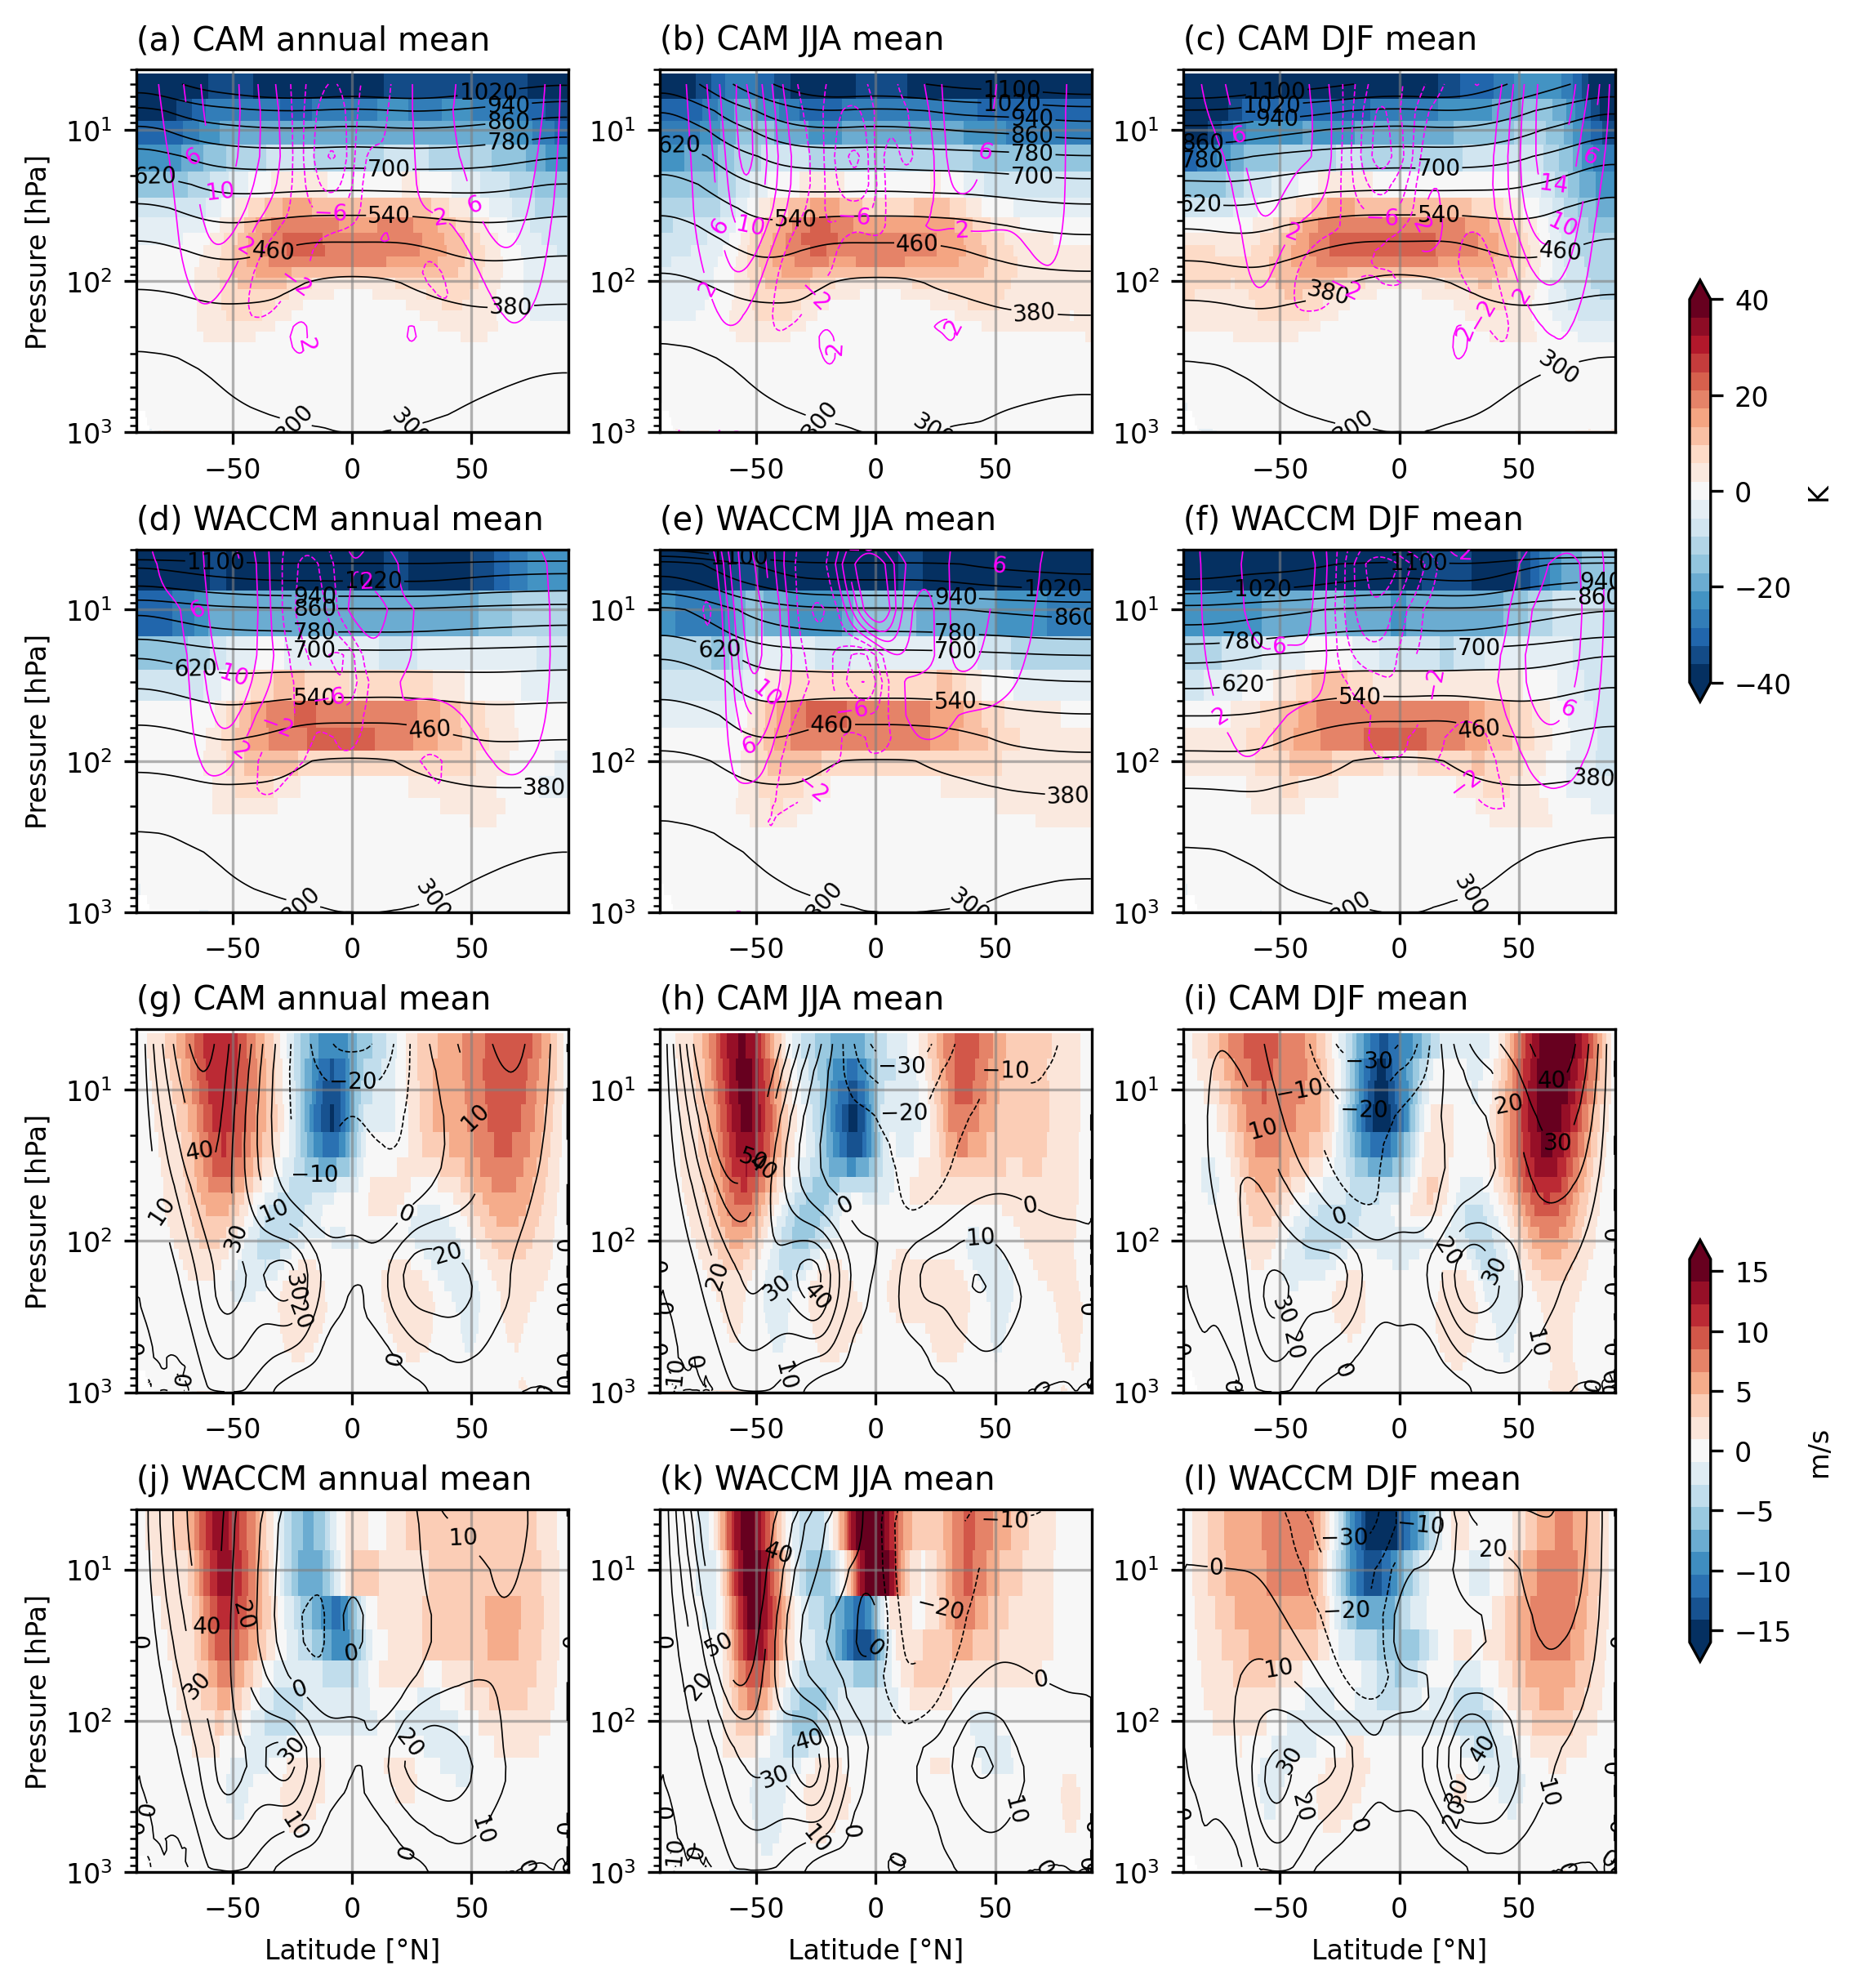
\includegraphics[width=\linewidth]{/Users/Simone/Documents/Uni/Master/Y2/Thesis/Paper_imgs/png/th_U_full.png}
	\caption{(a-f): Potential temperature anomaly for (a-c) CAM and (d-f) WACCM, annual, JJA and DJF mean shown for both models. Reference potential temperature shown in black contours, zonal wind anomalies shown in magenta contours. (g-l): Zonal mean zonal wind anomaly for WACCM and CAM analogous to (a-f), Reference zonal wind shown in black contours.}
	\label{fig:th_U}
\end{figure} 

The zonal mean potential temperature and zonal mean zonal wind are shown in Figure \ref{fig:th_U}, we learn:

\begin{itemize}
	\item potential temperature shows heating in the same pattern as the aerosol distribution. Cooling in the upper stratosphere from CO$_2$ still visible as this is RCP8.5 background. No significant heating shown below 200 hPa supporting notion that emulator works for SAI 2020 scenario. 
	\item Zonal wind shows increase most notably where the temperature gradient is increased, around 60°N/S, conclusion: thermal wind increased.
	\item Zonal wind/thermal wind increase mostly in winter hemisphere, related to Polar Night Jet. 
\end{itemize}

TO DO: aerosol figure!!!!!

\subsection{Supplementary material}

\subsubsection{Absolute model differences}
\begin{figure}[H]
	\centering
	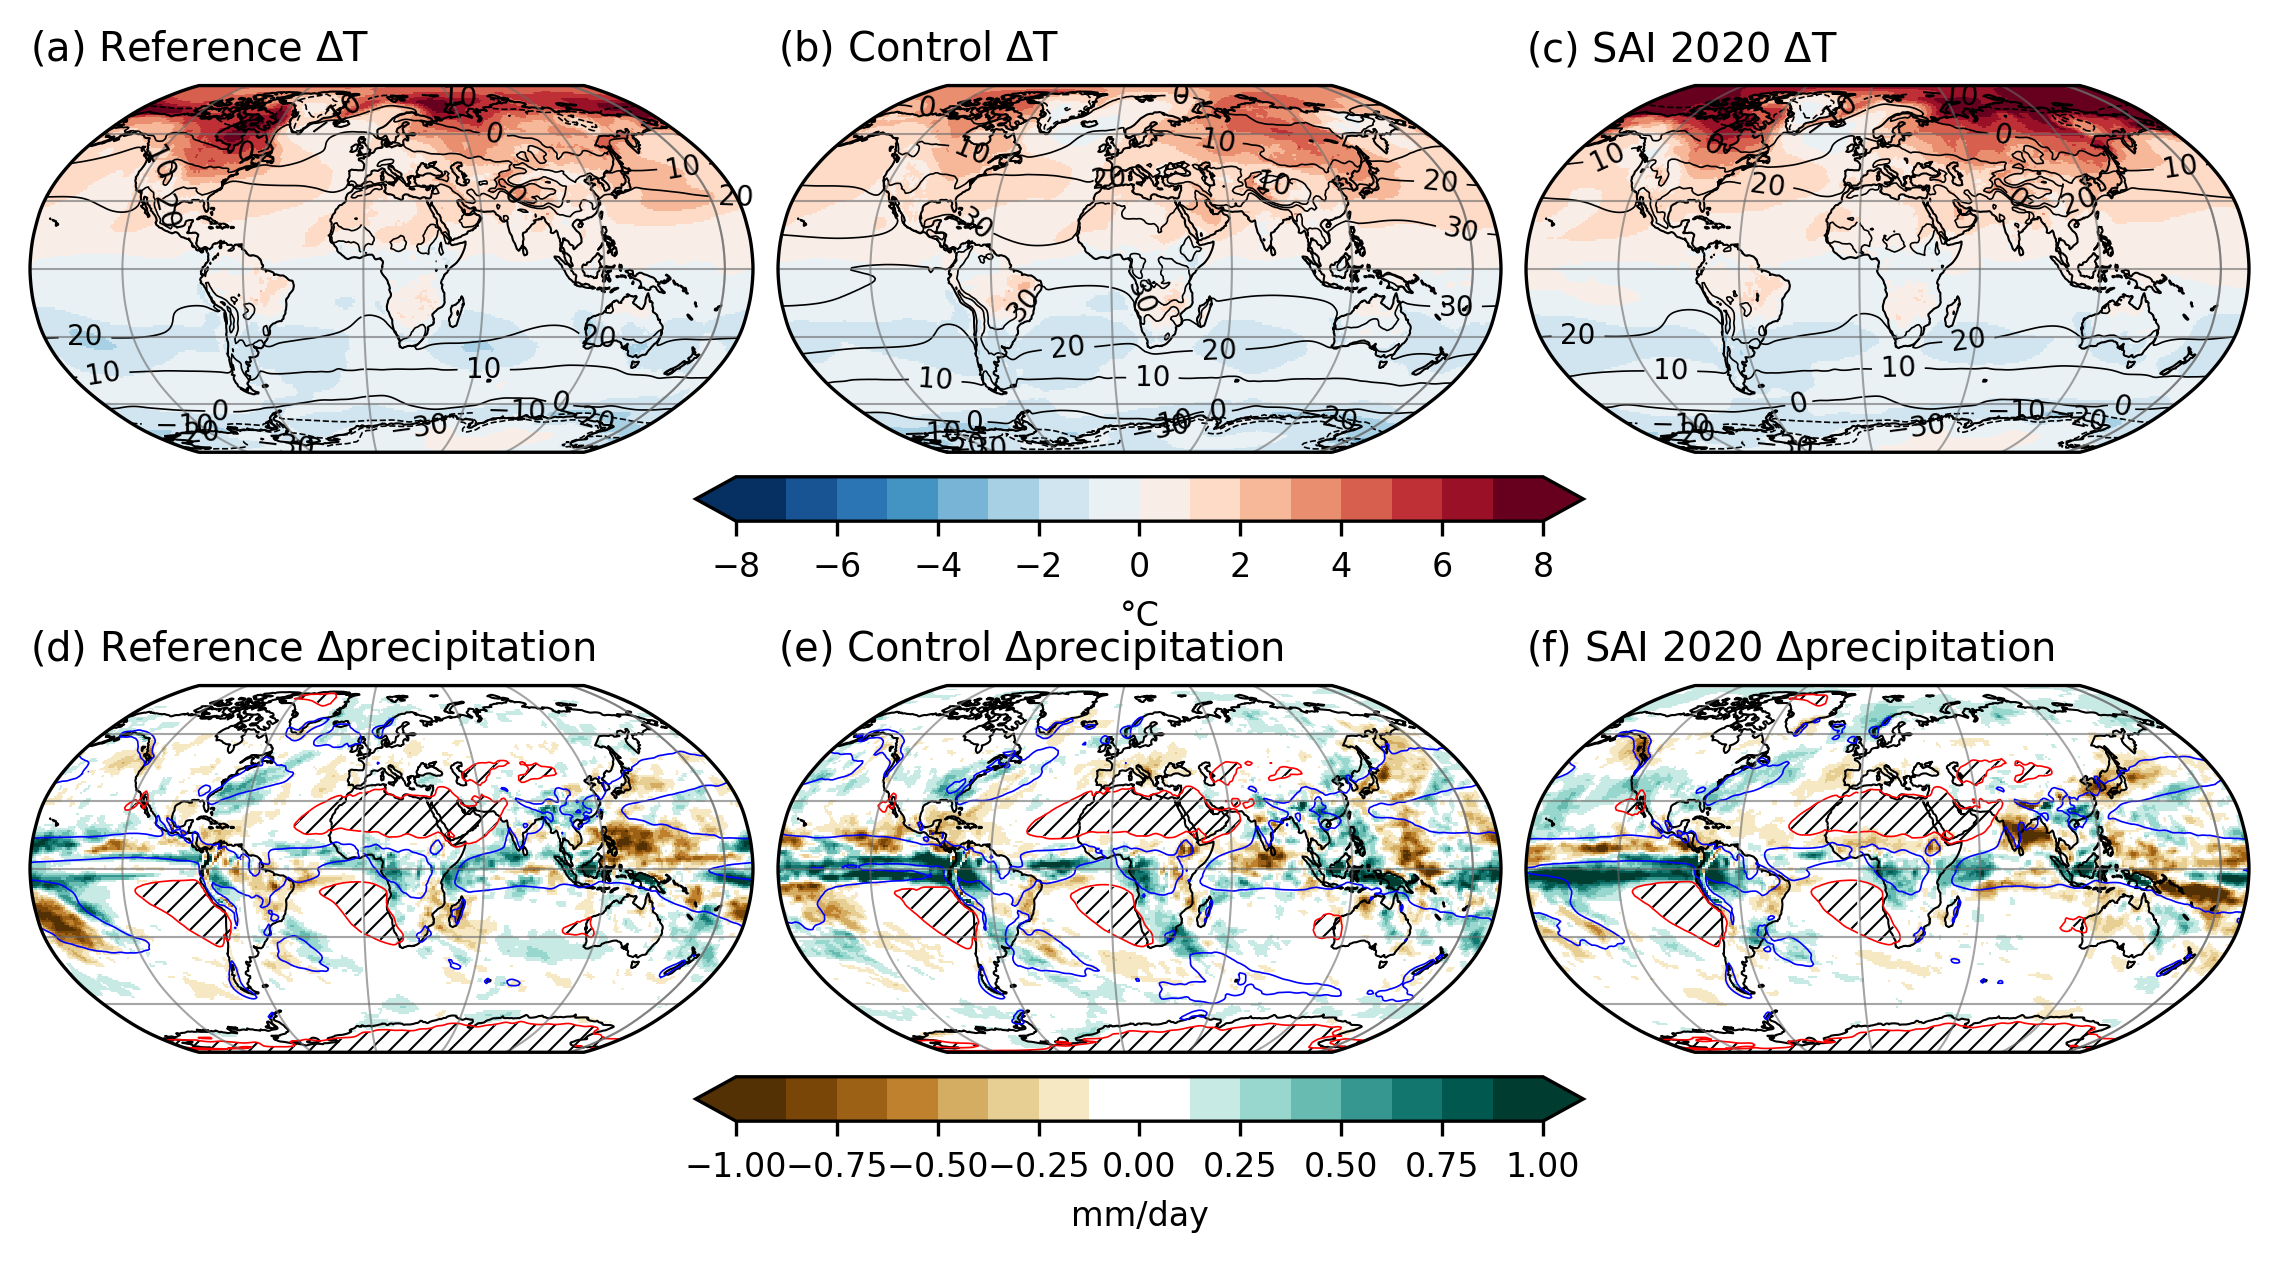
\includegraphics[width=\linewidth]{/Users/Simone/Documents/Uni/Master/Y2/Thesis/Paper_imgs/png/CAM_WACCM.png}
	\caption{(a-c): Reference, Control and SAI 2020 CAM-WACCM reference height temperature differences, contours show WACCM temperature in 10°C intervals. (d-e): Analogous to (a-c) for precipitation, 4 mm/day in blue contours, $<0.3$ mm/day in red contours with hatching.}
	\label{fig:abs_diff}
\end{figure}

TO DO: precipitation op \% schaal, checken of alles goedgegaan is?

\subsubsection{Precipitation Anomaly}

\begin{figure}[H]
	\centering
	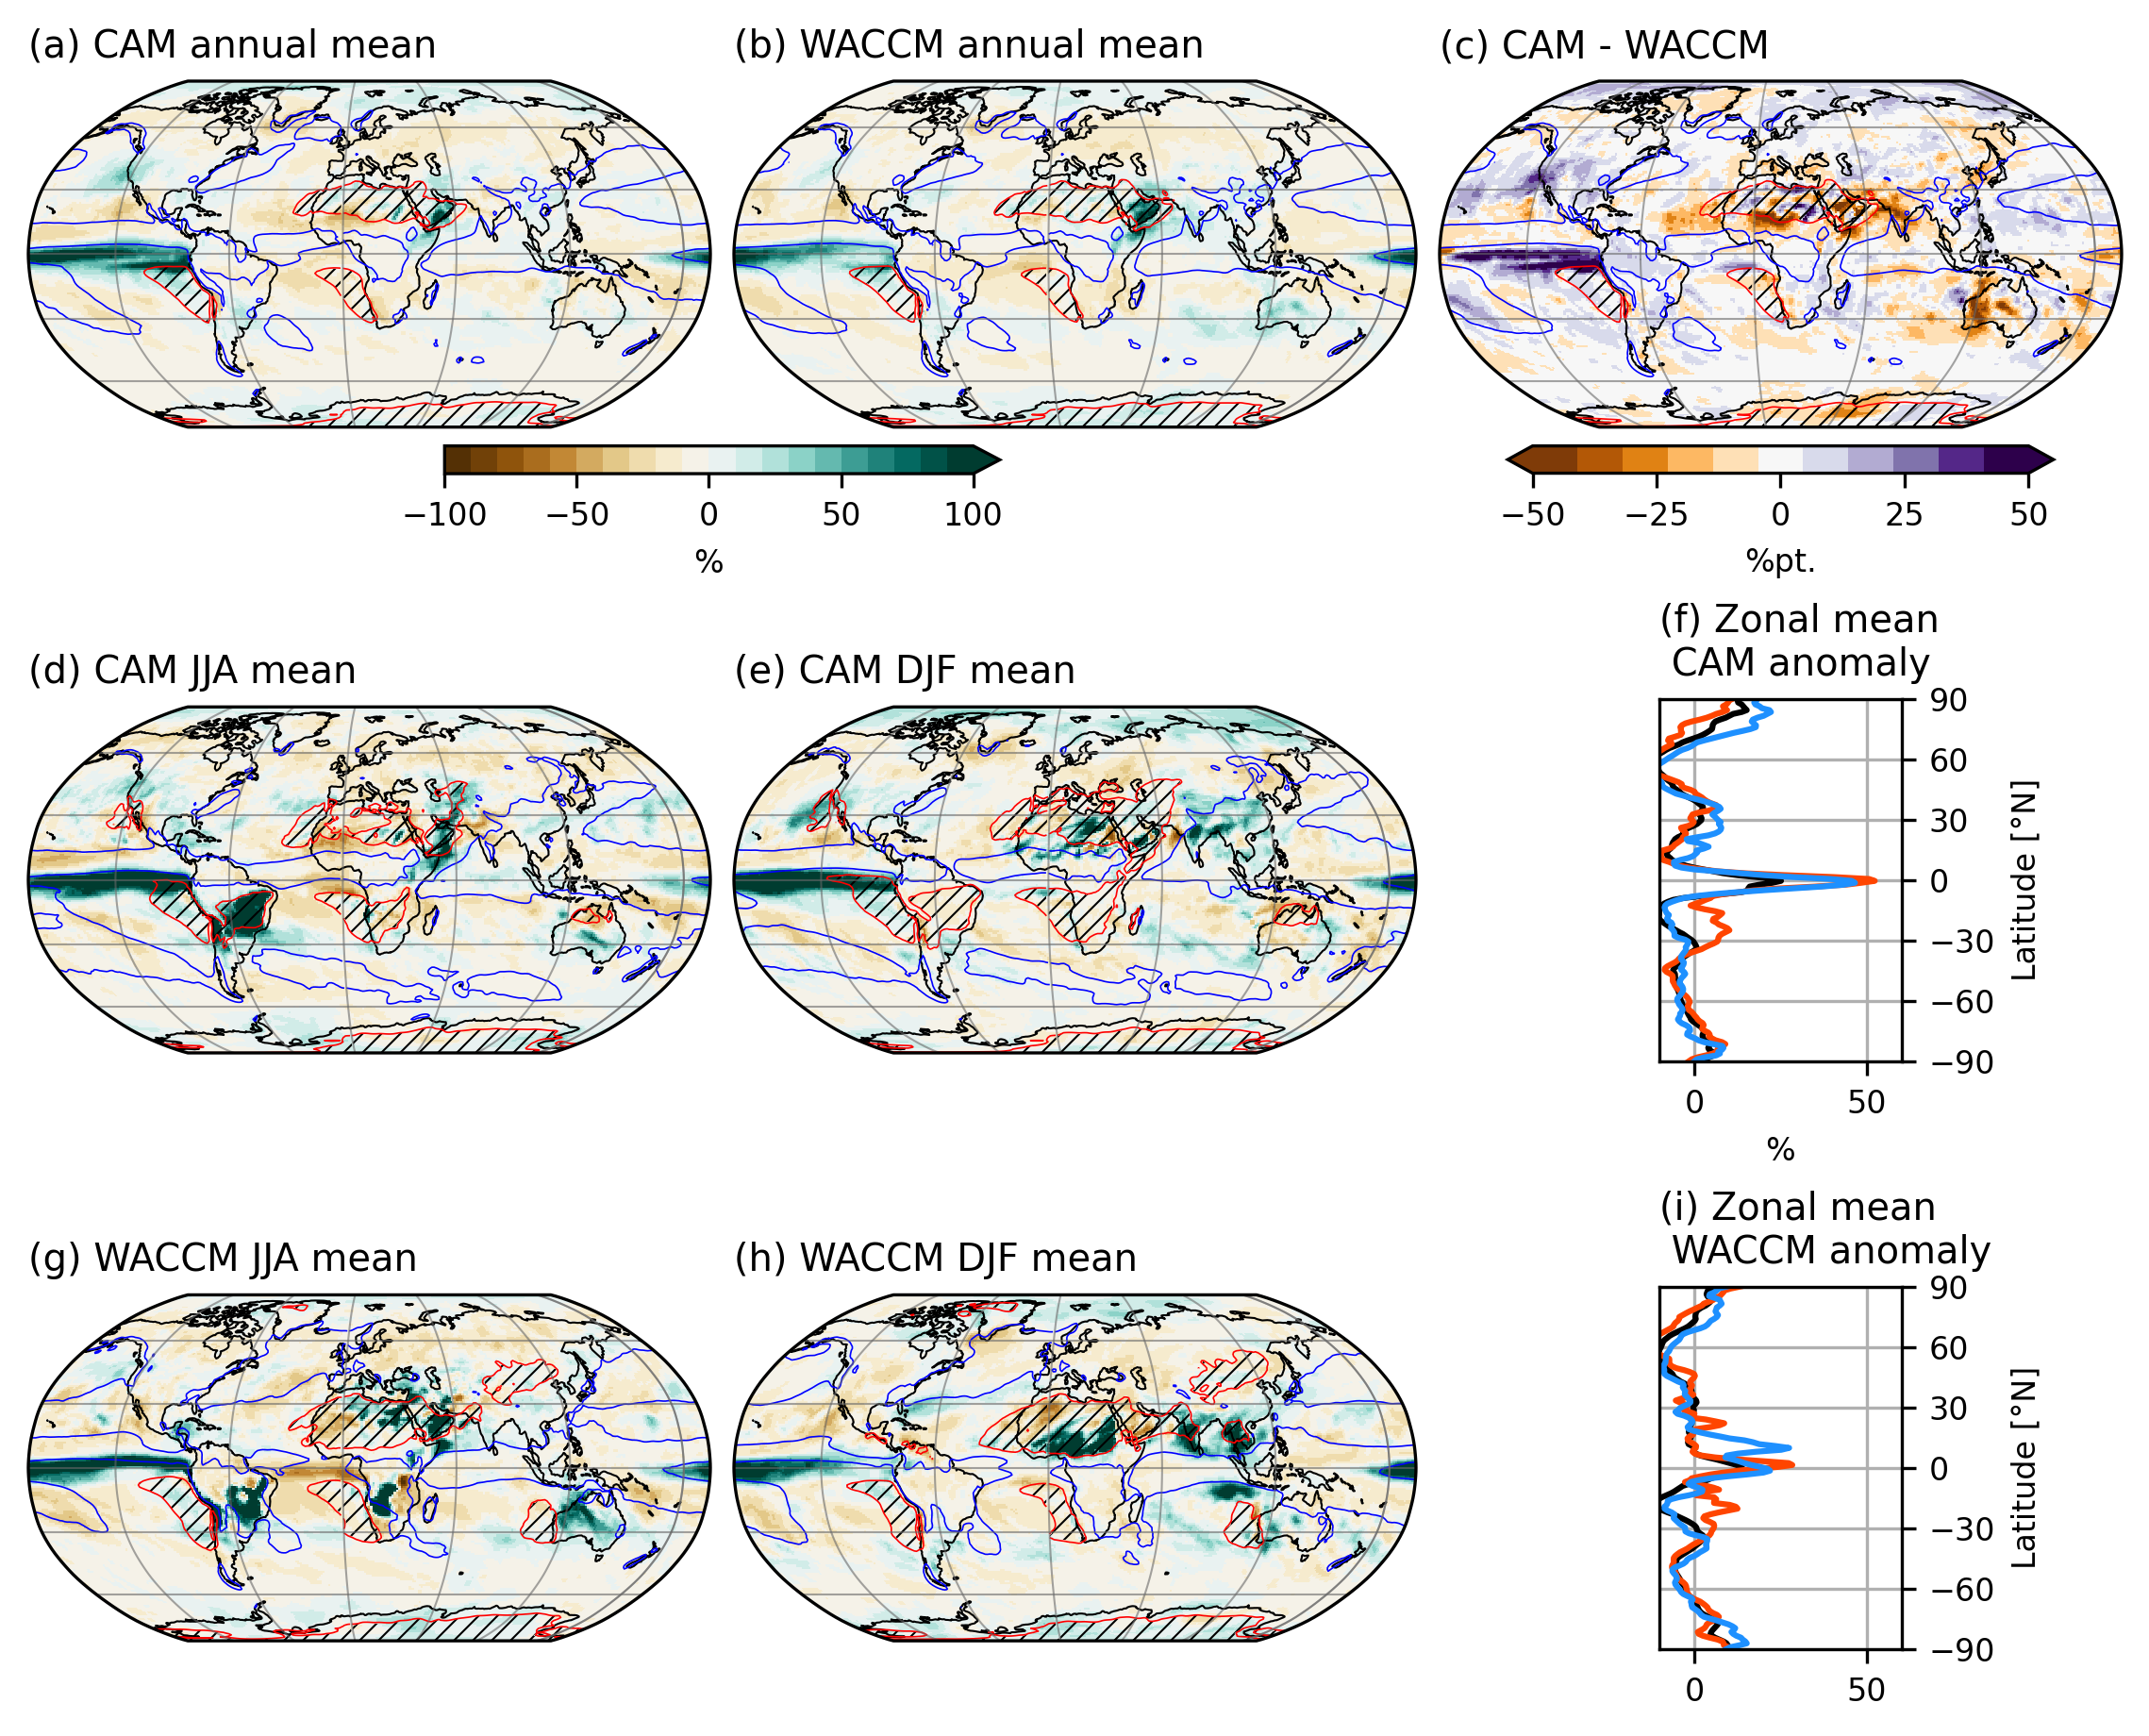
\includegraphics[width=\linewidth]{/Users/Simone/Documents/Uni/Master/Y2/Thesis/Paper_imgs/png/PRECT_20ref.png}
	\caption{(a,b): Annual mean precipitation anomalies of SAI 2020 compared to Reference in (a) CAM and (b) WACCM. Reference mean precipitation shown, 4 mm/day in blue, $<0.3$mm/day in red with hatching. (c): Difference between CAM and WACCM precipitation anomalies. WACCM Control mean precipitation again shown as in (b). (d,e): CAM anomalies as in (a,b) for (d) JJA and (e) DJF. (f): CAM zonal average precipitation anomaly as in (a,b), annual mean anomaly in black, JJA anomaly in red, DJF anomaly in blue. (g,h,i): analogous to (d,e,f) for WACCM.}
	\label{fig:PRECT}
\end{figure}

The annual mean precipitation anomalies are shown in Figure \ref{fig:PRECT}.

